%----------------------------------------------------------------------------------------
%	PACKAGES AND OTHER DOCUMENT CONFIGURATIONS
%----------------------------------------------------------------------------------------

%\documentclass[a4paper]{scrartcl}
\documentclass[a4paper]{scrreprt}
%\documentclass[12pt,a4paper,oneside,openright]{scrreprt}

\usepackage[T1]{fontenc}
\usepackage[french]{babel}
\usepackage[utf8x]{inputenc}

\usepackage{lmodern}
\usepackage{amsmath}
\usepackage{amssymb}
\usepackage{caption}
\usepackage{subcaption}
\usepackage{graphicx}
\usepackage{microtype}
\usepackage{minted}
\usepackage{babel}
\usepackage[babel]{csquotes}
\usepackage[section]{placeins}
\usepackage[]{units}
\usepackage{lastpage}
\usepackage[automark, headsepline, plainheadsepline,footsepline, plainfootsepline]{scrpage2}
\usepackage{array}
\usepackage{hyperref}
\usepackage{scrhack}
\usepackage{enumitem}
\usepackage{pdfpages}
\usepackage{glossaries}
\usepackage{fullpage}
\usepackage{eso-pic}

\setminted{
  autogobble=true,
  breakautoindent=false,
  breaklines=true,
  breakbytoken=true,
  frame=single,
  linenos=true,
  %showspaces=true,
}

\setlength{\headsep}{1cm} %comment this line for delete space between header and text block
%\setlength{\headheight}{1.1\baselineskip}

\newcommand{\HRule}{\rule{\linewidth}{0.2mm}} % Defines a new command for the horizontal lines, change thickness here

\newcommand{\blap}[1]{\vbox to 0pt{#1\vss}}
\newcommand\AtUpperLeftCorner[3]{%
  \put(\LenToUnit{#1},\LenToUnit{\dimexpr\paperheight-#2}){\blap{#3}}%
}
\newcommand\AtUpperRightCorner[3]{%
  \put(\LenToUnit{\dimexpr\paperwidth-#1},\LenToUnit{\dimexpr\paperheight-#2}){\blap{\llap{#3}}}%
}

\renewcommand\listoflistingscaption{Table des codes}

\makeatletter
\title{Gestion de Tutoring en ligne} \let\Title\@title
\author{Miguel \textsc{Pereira Vieira}}\let\Author\@author

\pagestyle{scrheadings}

\clearscrheadings
\clearscrplain
\clearscrheadfoot

\ihead[\leftmark]{\leftmark}
\ohead[Travail de bachelor 2016-2017]{Travail de bachelor 2016-2017}
\ifoot[\Author]{\Author}
\ofoot[\pagemark/\pageref{LastPage}]{\pagemark/\pageref{LastPage}}
\makeatother

\makeglossaries
\newglossaryentry{sql}{name=SQL, description={Structured Query Language}}
\newglossaryentry{nosql}{name=No-SQL, description={Not only Structured Query Language}}
\newglossaryentry{bson}{name=BSON, description={Binary javaScript  Object Notation}}
\newglossaryentry{json}{name=JSON, description={JavaScript  Object Notation}}
\newglossaryentry{crud}{name=CRUD, description={Create Read Update Delete}}
\newglossaryentry{html}{name=HTML, description={HyperText Markup Language}}
\newglossaryentry{css}{name=CSS, description={Cascading Style Sheets}}
\newglossaryentry{php}{name=PHP, description={PHP Hypertext Preprocessor}}

\begin{document}
\begin{titlepage}
	\enlargethispage{2cm}
%----------------------------------------------------------------------------------------
%	HEADING SECTIONS
%----------------------------------------------------------------------------------------
	\AddToShipoutPicture{
        \AtUpperLeftCorner{1.5cm}{1cm}{
\includegraphics[width=5cm]{img/logo_hepia.jpg}}
        \AtUpperRightCorner{1.5cm}{1cm}{
\includegraphics[width=5cm]{img/logo_hes.png}}
    }
%----------------------------------------------------------------------------------------
%	TITLE SECTION
%----------------------------------------------------------------------------------------
\begin{center}
	\vspace*{1.5cm}
 
    { \huge \bfseries \Title}\\ % Title of your document
    \HRule \\[1.5cm]
    \vspace*{0.5cm}

    
\includegraphics[scale=0.2]{img/draft.png}\\[2.0cm] % Adding your description picture
    
    { \Large Thèse de Bachelor présentée par}\\[0.8cm]
    { \LARGE \textbf{Monsieur \Author}}\\[2cm]
    
    { \Large pour l'obtention du titre Bachelor of Science HES-SO en}\\[0.5cm]
    {\Large \textbf{Ingénierie des technologies de l’information avec orientation en logiciels et systèmes complexes}}\\[1cm]
    
    {\Large \textbf{Septembre 2017}} % Date, change the \today to a set date if you want to be precise
\end{center}

\vspace*{4cm} % Change size to keep end text on the title page

\begin{flushleft}
{ \Large Professeur HES reponsable TB}\\[0.2cm]
{ \Large \textbf{Yassin \textsc{Rekik}}}
\end{flushleft}
 
%----------------------------------------------------------------------------------------
\newpage
\end{titlepage}
\ClearShipoutPicture

%\includepdf[pages={1}]{test.pdf} %  Inclure un pdf dans cette page

\chapter*{Énoncé}
\section*{Descriptif}
Ce projet consiste à développer une plate-forme web pour la gestion de tutoring entre un répétiteur et son étudiant. La plate-forme doit permettre une inscription en tant que répétiteur ou étudiant. Selon ce choix là, les options possibles ne seront pas les mêmes en tenant compte qu'un répétiteur devra spécifier le(s) domaine(s) pour lesquels il souhaite donner un appui, d'autres critères permettront également de classer un répétiteur (prix, langue,...). Un étudiant devra fournir des informations basiques comme son âge, son adresse, sa langue, son degré scolaire.

À partir de là, la plate-forme doit pouvoir proposer des répétiteurs aux étudiants selon les critères qu'ils auront spécifiés. Par la suite, répétiteur et étudiant devront se mettre d'accord sur une date et heure qui leur convient pour se retrouver sur la plate-forme et commencer la session de tutoring qui propose un dialogue audio-visuel entre les deux personnes et un chat qui leur permettra de communiquer. Du contenu provenant de bases de données contenant des exercices, questions et autres techniques seront à la disposition du répétiteur s'il souhaite les proposer à son étudiant.

À la fin de la session l'étudiant doit pouvoir noter son répétiteur avec un système de point qui permettra de monter ou diminuer la côte du répétiteur.

\section*{Travail demandé}

\chapter*{Résumé}
\chapter*{Remerciements}

\tableofcontents

\listoffigures

\listoflistings

\printglossaries

\chapter{Introduction}
Dans ce projet ce que nous appelons \textit{tutoring} est la méthode d'enseignement entre un répétiteur et un étudiant.

\chapter{Analyse}
\section{Diagramme des cas d'utilisations}
On va commencer par regarder les cas d'utilisations de chacun des acteurs de notre site web pour comprendre qu'elles sont les fonctionnalités de notre plate-forme et de quel manière on peut y accéder. De ce fait on aura une idée précise de ce que chaque type d'utilisateur pourra faire depuis notre application.
\subsection{Visiteur}
\begin{figure}[H]
  \centering
  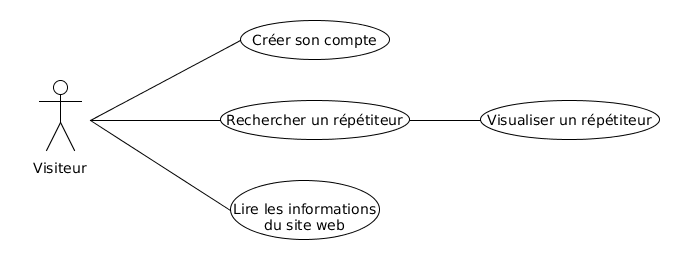
\includegraphics[width=\textwidth]{img/UseCase_Visiteur.png}
  \caption{Diagramme de cas d'utilisation pour les visiteurs}
  \label{fig:uc_visiteur}
\end{figure}

\subsection{Étudiant}
\begin{figure}[H]
  \centering
  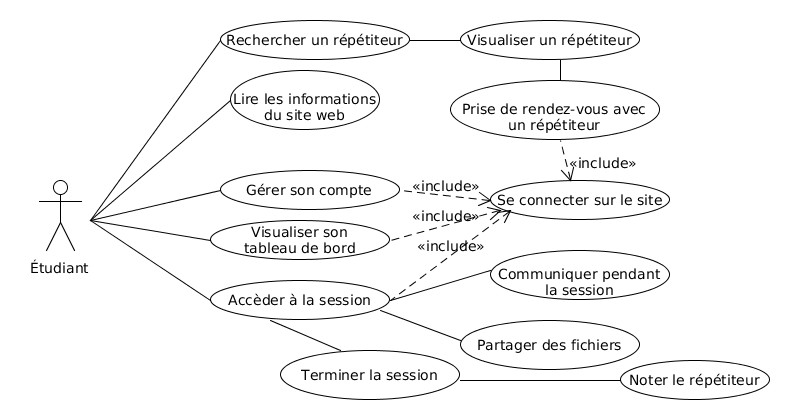
\includegraphics[width=\textwidth]{img/UseCase_Etudiant.png}
  \caption{Diagramme de cas d'utilisation pour les étudiants}
  \label{fig:uc_etudiant}
\end{figure}

\subsection{Parents}
\begin{figure}[H]
  \centering
  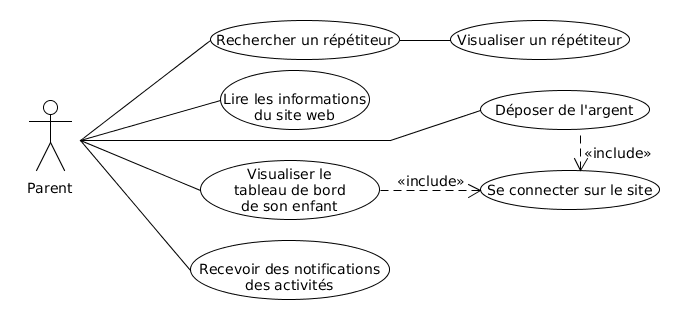
\includegraphics[width=\textwidth]{img/UseCase_Parent.png}
  \caption{Diagramme de cas d'utilisation pour les parents}
  \label{fig:uc_parent}
\end{figure}

\subsection{Répétiteur}
\begin{figure}[H]
  \centering
  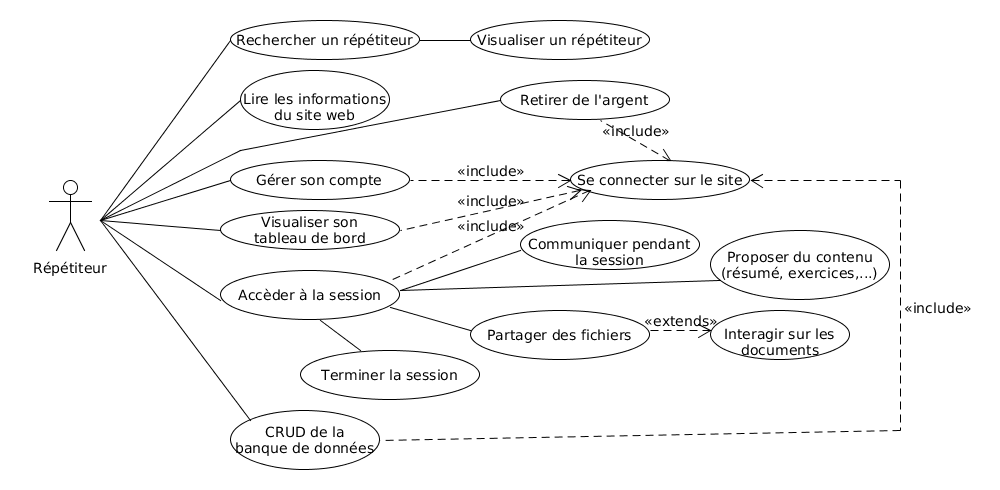
\includegraphics[width=\textwidth]{img/UseCase_Repetiteur.png}
  \caption{Diagramme de cas d'utilisation pour les répétiteurs}
  \label{fig:uc_repetiteur}
\end{figure}

\subsection{Administrateur}
\begin{figure}[H]
  \centering
  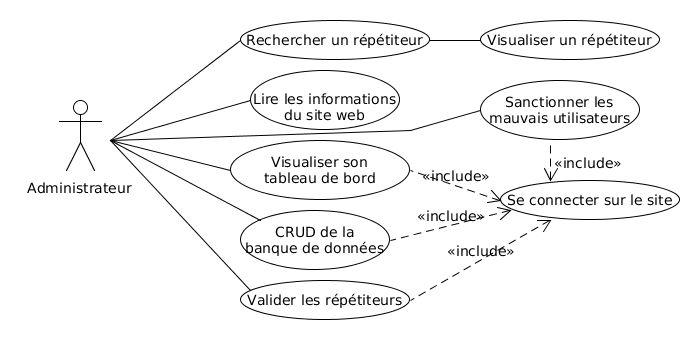
\includegraphics[width=\textwidth]{img/UseCase_Administrateur.png}
  \caption{Diagramme de cas d'utilisation pour les administrateurs}
  \label{fig:uc_administrateur}
\end{figure}


\section{Frontend}
Pour développer ce projet on a choisi d'utiliser une plate-forme web pour réaliser ce qui a été convenu. On va informer le lecteur sur les technologies utilisées pour réaliser la partie visuel de notre plate-forme.
\subsection{Technologies utilisées}
\subsubsection{Bootstrap(\gls{html}/\gls{css})}
Pour la réalisation du site web on a choisi d'utiliser le framework Bootstrap. Ce framework permet de se baser sur plusieurs types de templates et du coup d'avoir un site web avec un design sympathique sans avoir à trop se soucier des détails, c'était l'idéal pour ne pas perdre de temps avec le côté artistique du site web. De plus ce framework permet d'avoir un site web responsive ce qui implique que le site web sera visualisable sur un mobile et/ou une tablette sans avoir à changer du code par rapport à la version desktop.
\subsubsection{\gls{php}}
On utilise le \gls{php} pour effectuer des traitements sur nos pages web avant de récupérer les valeurs à l'aide de jQuery
\subsubsection{JavaScript}
Le langage JavaScript va permettre de rendre les pages notre site web dynamique.
\subsubsection{jQuery}
Le jQuery va nous permettre de récupérer les informations de nos formulaires et de communiquer avec notre serveur. Les résultats renvoyés par le serveur sont au format \gls{json} et seront traités par jQuery également avant d'être affiché sur la page.

\section{MongoDB}
\subsection{Introduction}
MongoDB est une base de données de type \gls{nosql}. Une base de données du type \gls{nosql} est un système qui n'applique pas le schéma classique que l'on appelle <<relationnelle>>.

MongoDB est une base de données orienté pour le traitement de grandes quantités de données. Cette base n'as plus un référencement par table et clé étrangère entre ces tables mais plutôt un seul endroit où tout est stocké dans un seul document. Ces documents utilise le format \gls{bson}\footnote{Un format basé sur du \gls{json} avec plus de types de valeur} pour le stockage de leur données.

MongoDB est une base de données qui permet la communication avec énormément de langage: C, C++, Go, Java, JavaScript, NodeJs, PHP et bien d'autres...
\subsection{Installation}
Pour l'installation de MongoDB, le plus simple est de consulter leur documentation officielle qui est spécifiée pour plusieurs systèmes d'exploitation, la démarche que je vais préciser par la suite est utilisé pour une distribution Ubuntu 16.04 et comprend 4 étapes:

\begin{enumerate}
\item Importer la clé publique du système de gestion de paquet\\
\begin{minted}{Shell}
sudo apt-key adv --keyserver hkp://keyserver.ubuntu.com:80 --recv 0C49F3730359A14518585931BC711F9BA15703C6
\end{minted}

\item Créer une liste de fichier pour MongoDB\\
\begin{minted}{Shell}
echo "deb [ arch=amd64,arm64 ] http://repo.mongodb.org/apt/ubuntu xenial/mongodb-org/3.4 multiverse" | sudo tee /etc/apt/sources.list.d/mongodb-org-3.4.list
\end{minted}

\item Mettre à jour notre gestionnaire de paquets\\
\begin{minted}{Shell}
sudo apt-get update
\end{minted}

\item Installer le paquet MongoDB\\
\begin{minted}{Shell}
sudo apt-get install -y mongodb-org
\end{minted}
\end{enumerate}

\subsection{Termes utilisés}
Avant de commencer à montrer des exemples de requêtes sur une base de données MongoDB, il peut être utile de voir l'équivalence des termes utilisés en \gls{sql} et leur synonyme dans le monde de MongoDB. Le tableau~\ref{table:termes} démontre cela:
\begin{table}[H]
	\centering
	\begin{tabular}{| c | c |}	
    	\hline
        SQL & MongoDB \\ \hline
        database & database \\ \hline
        table & collection \\ \hline
        row & document ou BSON document \\ \hline
        column & field \\ \hline
        index & index \\ \hline 
        table joins & \$lookup \\ \hline 
        primary key & primary key \\ \hline 
  	\end{tabular}
  	\caption{Équivalence des termes entre SQL et MongoDB}
    \label{table:termes}
\end{table}
\subsection{Fonctionnement avec Node.js}
Pour ce projet, le serveur sera développé à l'aide de Node.js ce qui implique que les exemples qui suivront seront développés en JavaScript pour s'assurer de la compatiblité.

Les sous-chapitres suivants vont démontrer comment éxecuter la base de données MongoDB ainsi qu'un exemple de requêtes d'insertion, lecture et suppression sur MongoDB à l'aide de Node.js
\subsubsection{Lancement}
Après avoir installé MongoDB il faut savoir que les paramètres par défaut peuvent être modifiés sur le fichier se trouvant à l'arborescence suivante: \mintinline{shell}|/etc/mongod.conf| \\
Dans notre cas la base de données sera lancé en localhost sur le port 27017. Pour démarrer la base de données il faudra lancer la commande suivante:\\
\begin{listing}[H]
	\begin{minted}{shell}
		sudo mongod --dbpath=/data/db
	\end{minted}
	\caption{Lancement de MongoDB}
	\label{lst:start_mongoDB}
\end{listing}
L'élévation de privilège est obligatoire car la base de données écrit dans des dossiers protégés, ensuite l'option dbpath est à spécifier au premier lancement, cet emplacement indique où seront stockées les données et d'autres permissions qui proviennent de MongoDB.

\subsubsection{Insertion}
\begin{listing}[H]
	\begin{minted}{JavaScript}	
      var insertDocuments = function(db, callback) {
        // Get the documents collection
        var collection = db.collection('table');
        // Insert some documents
        collection.insertMany([
          {a : 1}, {a : 2}, {a : 3}
        ], function(err, result) {
          assert.equal(err, null);
          assert.equal(3, result.result.n);
          assert.equal(3, result.ops.length);
          console.log("Inserted 3 documents into the collection");
          callback(result);
        });
      };
	\end{minted}
	\caption{Fonction d'insertion de document}
	\label{lst:insert_mongoDB}
\end{listing}
Dans cet exemple on utilise une fonction qui va ajouter 3 valeurs statiques à notre base de données MongoDB en utilisant la fonction \mintinline{javascript}|insertMany| dans la collection nommé \textit{table}.
\subsubsection{Lecture}
\begin{listing}[H]
	\begin{minted}{javascript}	
     var findDocuments = function(db, callback) {
        // Get the documents collection
        var collection = db.collection('table');
        // Find some documents
        collection.find({}).toArray(function(err, docs) {
          assert.equal(err, null);
          console.log("Found the following records");
          console.log(docs)
          callback(docs);
        });
      };
	\end{minted}
	\caption{Fonction de lecture de document}
	\label{lst:read_mongoDB}
\end{listing}
Pour cette exemple on a une fonction qui récupère tous les documents de la collection \textit{table} et qui les affiches. La ligne 5 contient cette méthode \mintinline{javascript}|find| où on lui précise de n'appliquer aucun filtre sur sa recherche.

\subsubsection{Suppression}
\begin{listing}[H]
	\begin{minted}{javascript}	
     var removeDocument = function(db, callback) {
      // Get the documents collection
      var collection = db.collection('table');
      // Delete document where a is 3
      collection.deleteMany({ a : 3 }, function(err, result) {
        assert.equal(err, null);
        console.log("Removed the document with the field a equal to 3");
        callback(result);
      });    
    };
	\end{minted}
	\caption{Fonction de suppression de document}
	\label{lst:delete_mongoDB}
\end{listing}
Dans ce dernier exemple, le code est très semblable aux deux autres la seule différence est la méthode que l'on appelle à la ligne 5 où l'on précise de supprimer tous les éléments de la collection qui ont une entrée équivalente à <<a>> pour le champ du document et <<3>> comme valeur.


\chapter{Conception}
\section{Architecture logiciel}

\section{Backend}
La partie intelligence de notre projet contiendra un serveur ainsi qu'une base de données, ces éléments seront expliqués en détail dans ce chapitre. La base de données contiendra les données d'un utilisateur, les différents cours et toute la partie organisationnel du site web mais elle contient également toutes les données liées à notre banque de données pour offrir du contenu intéressant à nos duos répétiteur/étudiant. Le serveur sera l'intermédiaire entre notre client web et la base de données.
\subsection{Serveur}


\section{Interfaces}

\section{Base de données}

\begin{listing}[H]
\begin{minted}{json}
  {
    "_id" : ObjectId("592be46ce69da639351f1743"),
    "prenom" : "MyFirstname",
    "nom" : "MyName",
    "email" : "email@hepia.com",
    "pseudo" : "Pseudonyme",
    "password" : "7110eda4d09e062aa5e4a390b0a572ac0d2c0220",
    "canton" : "Genève",
    "soldes" : 0,
    "type" : "Coach",
    "emailParent" : null,
    "diplomes" : [ 
        "dipl_Pseudonyme_1.pdf", 
        "dipl_Pseudonyme_2.pdf"
    ],
    "tarif" : "42",
    "img_profil" : null,
    "isValid" : false,
    "isOnline" : false,
    "matieres" : [ 
        "Arts visuels", 
        "Biologie"
    ]
}
\end{minted}
\caption{Collection t\_users}
\label{lst:col_users}
\end{listing}


\section{Algorithmes utilisés}

\chapter{Réalisation}
\chapter{Tests}

\chapter{Conclusion}

\chapter{Sources}
\begin{itemize}[label=\textbullet]
\item Documentation de MongoDB: \url{https://docs.mongodb.com/}
\item Tutoriel pour protocole WebRTC: \url{https://www.html5rocks.com/en/tutorials/webrtc/basics/}
\item Documentation du framework Express: \url{http://expressjs.com/fr/}
\item Recupérer un fichier via jQuery: \url{https://www.mkyong.com/jquery/jquery-ajax-submit-a-multipart-form/}
\item Documentation de PeerJS: \url{http://peerjs.com/docs/}
\subsection*{Autoriser le cross-domain}
\item \url{https://buzut.fr/xhr-cross-domain-avec-node-js/}
\item \url{https://www.npmjs.com/package/cors/}
\end{itemize}


\end{document}